\documentclass[journal,12pt,twocolumn]{IEEEtran}

\usepackage{setspace}
\usepackage{gensymb}
\singlespacing
\usepackage[cmex10]{amsmath}

\usepackage{amsthm}

\usepackage{mathrsfs}
\usepackage{txfonts}
\usepackage{stfloats}
\usepackage{bm}
\usepackage{tcolorbox}
\usepackage{cite}
\usepackage{cases}
\usepackage{subfig}
\usepackage[T1]{fontenc}
\usepackage{inconsolata}

\usepackage{longtable}
\usepackage{multirow}

\usepackage{enumitem}
\usepackage{mathtools}
\usepackage{steinmetz}
\usepackage{tikz}
\usepackage{circuitikz}
\usepackage{verbatim}
\usepackage{tfrupee}
\usepackage[breaklinks=true]{hyperref}
\usepackage{graphicx}
\usepackage{tkz-euclide}
\usetikzlibrary{positioning}

\usetikzlibrary{calc,math}
\usepackage{listings}
    \usepackage{color}                                            %%
    \usepackage{array}                                            %%
    \usepackage{longtable}                                        %%
    \usepackage{calc}                                             %%
    \usepackage{multirow}                                         %%
    \usepackage{hhline}                                           %%
    \usepackage{ifthen}                                           %%
    \usepackage{lscape}     
\usepackage{multicol}
\usepackage{chngcntr}

\DeclareMathOperator*{\Res}{Res}

\renewcommand\thesection{\arabic{section}}
\renewcommand\thesubsection{\thesection.\arabic{subsection}}
\renewcommand\thesubsubsection{\thesubsection.\arabic{subsubsection}}

\renewcommand\thesectiondis{\arabic{section}}
\renewcommand\thesubsectiondis{\thesectiondis.\arabic{subsection}}
\renewcommand\thesubsubsectiondis{\thesubsectiondis.\arabic{subsubsection}}


\hyphenation{op-tical net-works semi-conduc-tor}
\def\inputGnumericTable{}                                 %%

\lstset{
%language=C,
frame=single, 
breaklines=true,
columns=fullflexible
}
\begin{document}


\newtheorem{theorem}{Theorem}[section]
\newtheorem{problem}{Problem}
\newtheorem{proposition}{Proposition}[section]
\newtheorem{lemma}{Lemma}[section]
\newtheorem{corollary}[theorem]{Corollary}
\newtheorem{example}{Example}[section]
\newtheorem{definition}[problem]{Definition}

\newcommand{\BEQA}{\begin{eqnarray}}
\newcommand{\EEQA}{\end{eqnarray}}
\newcommand{\define}{\stackrel{\triangle}{=}}
\bibliographystyle{IEEEtran}
\raggedbottom
\setlength{\parindent}{0pt}
\providecommand{\mbf}{\mathbf}
\providecommand{\pr}[1]{\ensuremath{\Pr\left(#1\right)}}
\providecommand{\qfunc}[1]{\ensuremath{Q\left(#1\right)}}
\providecommand{\sbrak}[1]{\ensuremath{{}\left[#1\right]}}
\providecommand{\lsbrak}[1]{\ensuremath{{}\left[#1\right.}}
\providecommand{\rsbrak}[1]{\ensuremath{{}\left.#1\right]}}
\providecommand{\brak}[1]{\ensuremath{\left(#1\right)}}
\providecommand{\lbrak}[1]{\ensuremath{\left(#1\right.}}
\providecommand{\rbrak}[1]{\ensuremath{\left.#1\right)}}
\providecommand{\cbrak}[1]{\ensuremath{\left\{#1\right\}}}
\providecommand{\lcbrak}[1]{\ensuremath{\left\{#1\right.}}
\providecommand{\rcbrak}[1]{\ensuremath{\left.#1\right\}}}
\theoremstyle{remark}
\newtheorem{rem}{Remark}
\newcommand{\sgn}{\mathop{\mathrm{sgn}}}
\providecommand{\abs}[1]{\left\vert#1\right\vert}
\providecommand{\res}[1]{\Res\displaylimits_{#1}} 
\providecommand{\norm}[1]{\left\lVert#1\right\rVert}
%\providecommand{\norm}[1]{\lVert#1\rVert}
\providecommand{\mtx}[1]{\mathbf{#1}}
\providecommand{\mean}[1]{E\left[ #1 \right]}
\providecommand{\fourier}{\overset{\mathcal{F}}{ \rightleftharpoons}}
%\providecommand{\hilbert}{\overset{\mathcal{H}}{ \rightleftharpoons}}
\providecommand{\system}{\overset{\mathcal{H}}{ \longleftrightarrow}}
	%\newcommand{\solution}[2]{\textbf{Solution:}{#1}}
\newcommand{\solution}{\noindent \textbf{Solution: }}
\newcommand{\cosec}{\,\text{cosec}\,}
\providecommand{\dec}[2]{\ensuremath{\overset{#1}{\underset{#2}{\gtrless}}}}
\newcommand{\myvec}[1]{\ensuremath{\begin{pmatrix}#1\end{pmatrix}}}
\newcommand{\mydet}[1]{\ensuremath{\begin{vmatrix}#1\end{vmatrix}}}
\numberwithin{equation}{subsection}

\makeatletter
\@addtoreset{figure}{problem}
\makeatother
\let\StandardTheFigure\thefigure
\let\vec\mathbf

\renewcommand{\thefigure}{\theproblem}

\def\putbox#1#2#3{\makebox[0in][l]{\makebox[#1][l]{}\raisebox{\baselineskip}[0in][0in]{\raisebox{#2}[0in][0in]{#3}}}}
     \def\rightbox#1{\makebox[0in][r]{#1}}
     \def\centbox#1{\makebox[0in]{#1}}
     \def\topbox#1{\raisebox{-\baselineskip}[0in][0in]{#1}}
     \def\midbox#1{\raisebox{-0.5\baselineskip}[0in][0in]{#1}}
\vspace{3cm}
\title{Assignment-1}
\author{Mohammed Sadiq - EE18BTECH11051}
\maketitle
\newpage
\bigskip
\renewcommand{\thefigure}{\theenumi}
\renewcommand{\thetable}{\theenumi}
Github repository
\begin{lstlisting}
https://github.com/Sadiq0123/C-and-DS/tree/main/Assignment-1
\end{lstlisting}
%

\section{\textbf{Problem}}

\textbf{Consider the following C program:}
\begin{tcolorbox}

\begin{verbatim}
#include <stdio.h> 

int counter = 0; 
int calc (int a, int b) { 
    int c; 
 
    counter++; 
    if (b==3) return (a*a*a); 
    else { 
        c = calc(a, b/3); 
        return (c*c*c); 
    } 
} 
 
int main (){ 
    calc(4, 81); 
    printf ("%d", counter); 
}
\end{verbatim}

\end{tcolorbox}

The output of this program is \_.


\section{\textbf{Solution}}
\textbf{Answer:} 4.
\\~\\
The variable \texttt{counter} is a global variable with initial value set to 0, and is incremented by 1 everytime the function \texttt{calc} is called.
\\~\\ 
The function \texttt{calc} returns $a^b$ only if $b$ is a power of 3; else the function returns nothing. The code behaves this way because eventually the function calls \texttt{calc(a, b/3)} where $b<3$, which leads to an infinite recursive call of \texttt{calc(a, 0)}. So, the stack overflow causes Segmentation Fault error during runtime.
\\~\\ 
If $b$ is valid, then \texttt{calc} recursively calls itself for $b/3$. So, the total number of times \texttt{counter} is incremented is $\log_3\brak{b}$ times. The following table shows the value of \texttt{counter} at every step.

\begin{center}
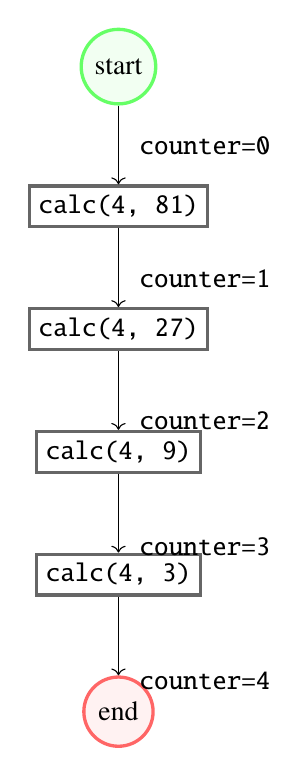
\begin{tikzpicture}[
roundnode/.style={circle, draw=green!60, fill=green!5, very thick, minimum size=7mm},
round2node/.style={circle, draw=red!60, fill=red!5, very thick, minimum size=7mm},
squarednode/.style={rectangle, draw=black!60, fill=white!5, very thick, minimum size=5mm},
]
%Nodes
\node[roundnode]        (start)                                 {start};
\node[squarednode]      (first)        [below=of start]         {\texttt{calc(4, 81)}};
\node[squarednode]      (second)       [below=of first]         {\texttt{calc(4, 27)}};
\node[squarednode]      (third)        [below=of second]        {\texttt{calc(4, 9)}};
\node[squarednode]      (fourth)       [below=of third]         {\texttt{calc(4, 3)}};
\node[round2node]        (end)          [below=of fourth]     {end};

%Lines
\draw[->] (start.south) -- (first.north);
\draw[->] (first.south) -- (second.north);
\draw[->] (second.south) -- (third.north);
\draw[->] (third.south) -- (fourth.north);
\draw[->] (fourth.south) -- (end.north);

%Text
\node[] at (1.1,-1) {\texttt{counter=0}};
\node[] at (1.1,-2.7) {\texttt{counter=1}};
\node[] at (1.1,-4.5) {\texttt{counter=2}};
\node[] at (1.1,-6.1) {\texttt{counter=3}};
\node[] at (1.1,-7.8) {\texttt{counter=4}};
\end{tikzpicture}
% \begin{tabular}{ |c|c| } 
%  \hline
%  \texttt{calc(a, b)} & \texttt{counter} \\ 
%  \hline
%  \texttt{calc(4, 81)} & \texttt{1} \\
%  \texttt{calc(4, 27)} & \texttt{2} \\
%  \texttt{calc(4, 9)} & \texttt{3} \\
%  \texttt{calc(4, 3)} & \texttt{4} \\
%  \hline
% \end{tabular}
\end{center}

As $\log_3\brak{81} = 4$, the output of the code would be equal to 4. 
\\~\\
The general mathematical relation between input \texttt{(a, b)} and output \texttt{counter} is:

$\texttt{counter} = log_3\brak{b}$

\end{document}
